\documentclass[tikz,border=5pt]{standalone}
\begin{document}
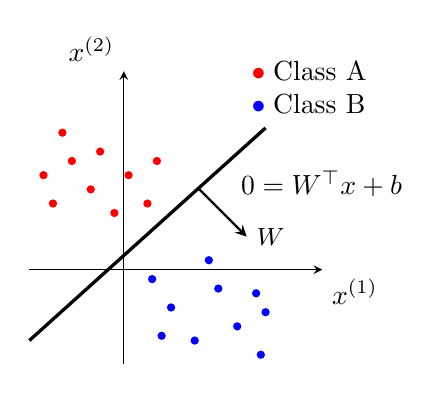
\begin{tikzpicture}[scale=0.6,>=stealth]
  % 坐标轴
  \draw[->] (-2,0) -- (4.2,0) node[below right] {$x^{(1)}$};
  \draw[->] (0,-2) -- (0,4.2) node[above left]  {$x^{(2)}$};

  % 决策边界:y = W^T x + b = 0
  \draw[very thick] (-2,-1.5) -- (3,3)
    node[pos=0.85, below right] {$0 = W^{\top}x + b$};

  % 红色点(左上区域)
  \begin{scope}[shift={(1.3,-0.5)}]
    \foreach \P in {
    (-3,2.5), (-2.8,1.9), (-2.4,2.8), (-2,2.2), 
    (-1.8,3.0), (-1.2,2.5), (-0.8,1.9), (-2.6,3.4), 
    (-1.5,1.7), (-0.6,2.8)}
    \fill[red] \P circle (2.5pt);
  \end{scope}

  % 蓝色点(右下区域)
  \begin{scope}[shift={(0,1.4)}]
    \foreach \P in {
    (3,-2.3), (2.8,-1.9), (2.4,-2.6), (2,-1.8), 
    (1.5,-2.9), (1.0,-2.2), (0.6,-1.6), (2.9,-3.2), 
    (1.8,-1.2), (0.8,-2.8)}
    \fill[blue] \P circle (2.5pt);
  \end{scope}

  \draw[->,thick] (1.6,1.7)--++(1,-1) node[right] {\small$W$};
  

  % 可选:图例
  \draw (2.5,4.2) node[anchor=west] {\textcolor{red}{$\bullet$}\;Class A};
  \draw (2.5,3.5) node[anchor=west] {\textcolor{blue}{$\bullet$}\;Class B};
\end{tikzpicture}
\end{document}